\section{Artificial Intelligence}
\subsection{Overview} 
        After breaking the Enigma machine that was made by the Nazis for secure/encrypted communications in world war against the allies, Alan Turing once again changed the course of history by asking the following question "Can machines think?" in a paper he published in 1950 titled "Computing Machinery and Intelligence", this question is what gave rise to Artificial Intelligence, because all what artificial intelligence is trying to do is answer that question in the affirmative by trying to mimic human intelligence in machines ~\cite{ai} to do so Turing has put forward a test called "The Turing Test" which will be explained later. Because artificial intelligence is a concept that is  so broad and general people don't always agree on a definition, but we found that the below definition is a good enough explanation.
        
    \subsection{Definition}
        "Artificial intelligence (AI) is a wide-ranging branch of computer science concerned with building smart machines capable of performing tasks that typically require human intelligence." ~\cite{ai}

    \subsection{Turing Test}
        It is basically a test put forward by the mathematician Alan Turing to determine whether a machine is intelligent or not, the test goes as follows, "If a machine can engage in a conversation with a human without being detected as a machine, it has demonstrated human intelligence." ~\cite{turing}
    
    \subsection{The 4 Types of Artificial Intelligence}
        \begin{description} 
        \item[Reactive Machines] \hfill \\
            It is one of the most basic form of artificial intelligence because as the title suggests it only reacts to its surrounding environment, and does not use a memory to try and learn from past experience, so it is purely reactive which means that this type of artificial intelligence can only be responsible for a very narrow and specialized set of tasks, this narrowness can be looked at as a limitation but in fact it is what makes it special in being very trustworthy and error free. A famous example of this type would be the chess playing machine Deep Blue made by IBM in the 1990s which treats each move in the game as its own separate reality and doesn't rely on past moves ~\cite{ai}.
        \item[Limited Memory] \hfill \\
            It is a type of artificial intelligence that relies on memory and automatic training, which means learning from experience to try to make optimized decisions/predictions, the learning steps in this type can be looked at as a feedback loop (generate data, learn, make model, make predictions, accept feedback), there are 3 major models that utilize this type ~\cite{ai}: 
            \begin{itemize}
                \item Reinforcement learning: learning from trial and error.
                \item Long Short Term Memory (LSTM):  uses past data to make predictions, the more recent the data the more weight it has on making predictions.
                \item Evolutionary Generative Adversarial Networks (E-GAN):  this model grows constantly by putting 2 machines against each other, and they learn by bouncing information off of each other. 
            \end{itemize}
        \item[Theory of Mind] \hfill \\
            This is purely theoretical and technology is still not caught up to this, and it stipulates that machines would be able to understand how humans and animals think and feel and make decisions through self reflection ~\cite{ai}.
        \item[Self-awareness] \hfill \\
            After Theory of Mind is established, this is the next step, where machines become self-aware and comprehensive of its own existence by obtaining human level intelligence and consciousness ~\cite{ai}.
        \end{description}
    
    \subsection{Artificial Intelligence Categories}
        Generally speaking, there are 2 categories of artificial intelligence ~\cite{ai}

            \begin{description} 
            \item[Narrow artificial intelligence] \hfill \\
                Also known as "Weak artificial intelligence", it operates in a limited context and is often specialized in a single task such as : Google Search, Image Recognition, Self-Driving Cars...etc.
            \item[Artificial general intelligence] \hfill \\
                Also known as "Strong artificial intelligence", it is the kind of artificial intelligence we see in Science Fiction movies implemented in robots that have human level intelligence and that can apply its intelligence to solve any problem.
            \end{description}
\section{Machine Learning}
    \subsection{Overview}
        Machine learning is a subfield of artificial intelligence that has a human like ability to learn from past experience through statistics and data, and it has helped us solve difficult world problems ranging from medical problems to environmental issues, and the special thing about machine learning is its ability to solve these problems without being explicitly programmed to do so with the usual sequence of code lines that define normal (non-artificial intelligence) algorithms, but it relies on tacit knowledge (past experience) to try and find patterns and make predictions, humans use tacit knowledge all the time for example a person can't accurately explain how he preforms face recognition, but it is gained through the experience of observing that face numerous times in different angles and states~\cite{ml}.

    \subsection{Definition}
        "Machine learning is a subset of artificial intelligence that gives systems the ability to learn and optimize processes without having to be consistently programmed. Simply put, machine learning uses data, statistics and trial and error to “learn” a specific task without ever having to be specifically coded for the task."~\cite{ml}.

    \subsection{Types of Machine Learning Algorithms}
        There are 3 types ~\cite{ml}
        \begin{description}
        \item[Supervised Learning] \hfill \\
            Supervised machine learning algorithms provide a mathematical model that can make the connection between inputs and outputs of the training data (pre-labeled data) in the most optimized way so that when it is provided with new data, it can make very accurate predictions. Regression and classification are the most popular supervised algorithms.
        \item[Unsupervised Learning] \hfill \\
            Unsupervised algorithms take unlabeled input data and try to structure it in the form of clustering or grouping by taking into account commonalities or lack of commonalities.
        \item[Semi-Supervised Learning] \hfill \\
            This type falls in the middle, it is given labeled and unlabeled data with unlabeled being the bigger percentage than the algorithm is going to cluster the unlabeled data through the structure of the labeled data which offers a huge optimization for both sides, because supervised learning requires a huge size of labeled data which is usually done by human beings which means that it takes a lot of time and is bound to human error, and Unsupervised learning algorithms takes a lot of time also figuring out the connections in the raw unlabeled data.
        \end{description}

    \subsection{Examples and Applications}
        As mentioned in ~\cite{ml}
        \begin{description}
        \item [Financial Services] \hfill \\
            This industry is using machine learning almost in every aspect, because of its ability to speed up the financial processes and preform tasks that used to take humans days or weeks in merely seconds. Such as handling millions of transactions, recommending personal offers ... etc.
        \item [Healthcare] \hfill \\
            This industry is also relying a lot on machine learning because of its ability to discover new treatments and detect and predict diseases, a medical professional equipped with machine learning is far more proficient because he can access a patient's relevant medical history in blink of an eye rather than digging through files or contacting other departments in the hospital. Machine learning is predicted to save the medical field billions of dollars annually.
        \item [Social Media] \hfill \\
            This industry usually uses machine learning for 2 main reasons: strengthening the feel of connection between people and eliminating bad actors, it does the former by providing individualized recommendations to friends, pages, and communities based on a user's preference or activity history, and for the latter it tries to prevent fake news before it becomes a thing, block malicious users and scams when detecting abnormalities.

        \item [...etc] \hfill \\
        \end{description}

        \section{Deep Learning}
        \subsection{Overview}
            Yet again another subfield with great capabilities, although it seems to be a new concept, but it actually isn't as our professor Rahmoun Abdellatif once mentioned in a lecture talking about deep learning and neural networks, he said that the theoretical part was established a long time ago (1950's) but people back then didn't have the computational power to implement it, so it took quite some time for people to develop the necessary computational power to take on artificial neural networks and one of the scientists who made neural networks cool again is Geoffrey Hinton by demonstrating that a few of them could be trained using backpropagation for better shape recognition and word prediction and by 2012 deep learning is basically used everywhere ~\cite{dl}.
    
        \subsection{Definition}
            "Deep learning (sometimes known as deep structured learning) is a subset of machine learning, where machines employ artificial neural networks to process information. Inspired by biological nodes in the human body, deep learning helps computers to quickly recognize and process images and speech. Computers then "learn" what these images or sounds represent and build an enormous database of stored knowledge for future tasks. In essence, deep learning enables computers to do what humans do naturally- learn by immersion and example."~\cite{dl}
    
        \subsection{What Is Next?}
            Although deep learning has brought us many accomplishments, and it can be applied in various domains and when it is done right it can preform a certain task with super-human level but some scientists and researchers say it is only a small step in acquiring actual intelligent machines because it lacks the concept of abstract ideas and knowledge such as: what objects are?, chat they are for?, how to use them?...etc.
            And also the problem of "data" because deep learning requires a huge amount of pre labeled data to be trained which is not always available and public datasets won't cut it~\cite{dl}.
    
            And there are a lot of new concepts that are presenting promising results like "deep reinforcement learning" a combination of deep learning and reinforcement learning, and we can see this implemented in a software called AlphaGo and AlphaGo Zero, another research paper suggested  "Reward learning from human preferences and demonstrations" which basically means machines learn from observing humans play games which they say it works better than trial-and-error systems~\cite{dl}.
    
            \bigskip \textbf{other ideas that are worth mentioning} ~\cite{dl}
                \begin{description}
                \item [ONE-SHOT LEARNING and NAS (neural architecture search)] \hfill \\
                    One-shot learning means we need far fewer data to learn, and NAS means an algorithm finds the best neural network architecture to solve a problem, this combination is very promising.
                \item [GANS (Generative Adversarial Networks)] \hfill \\
                    A competition for deep learning which puts 2 networks against each other (a generator and a discriminator) you can think of it as a counterfeiter and a cop.
                \item [AUTOML] \hfill \\
                    Learn-to-learn, which basically means machine learning algorithms do the hard work of finding the design of the network and all we need to provide is data.
                \end{description}
    
    
    \section{Ai vs Machine Learning vs Deep Learning}
        After all what we have talked about it is obvious that the relationship between the three is an inclusion relationship, deep learning is a subset of machine learning which is a subset of artificial intelligence as shown in Figure ~\ref{fig:versus} .
    
    \begin{figure}[htbp]
    \begin{center}
    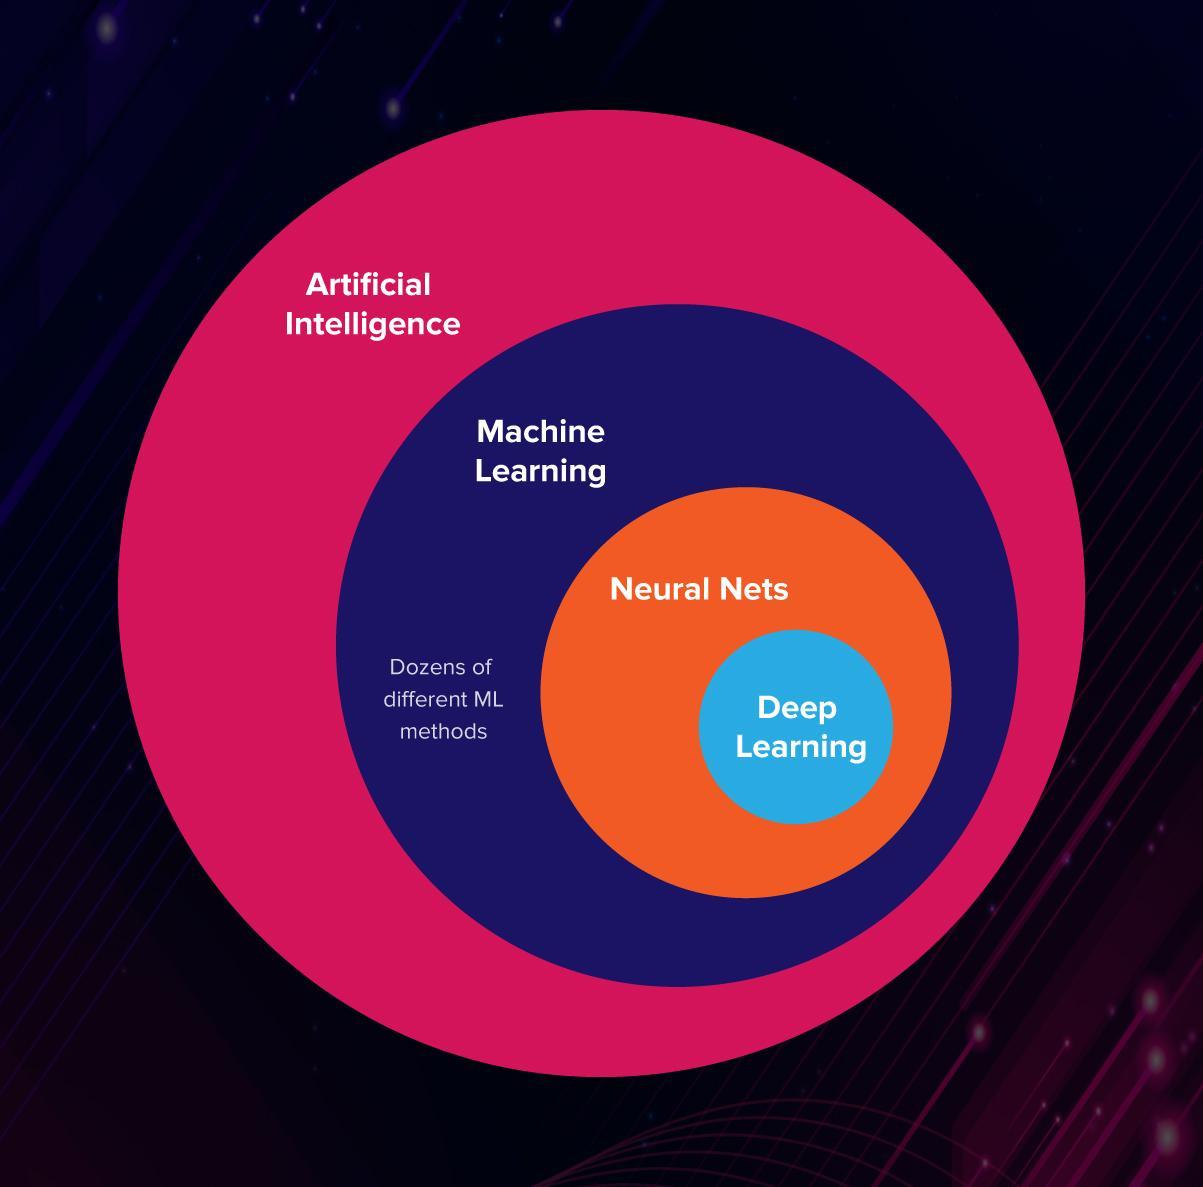
\includegraphics[width=10cm]{./chapter-02-general-ai-information/versus.jpg}
    \end{center}
    \caption{AI vs ML vs DL ~\cite{versus}}
    \label{fig:versus}
    \end{figure}
    
    



    \section{Computer Vision}
    \subsection{overview}
        Yet another subfield of artificial intelligence which is used to train machines to see, and by see we mean process analyze and extract useful information from images/videos just like us human beings, although our vision is far more advanced in many aspects because our brains were trained since birth to see, analyze objects, understand the distance and relationship between objects, attribute abstract information to objects...etc. But it is safe to say that machines can surpass our vision in certain specialized tasks because of their ability to process thousands of images/frames in a short period of time due to the constant increase in computational power especially (graphical processing). Computer vision is used in a wide variety of industries, and its market is estimated to reach 48.6 billion USD by 2022 ~\cite{machine-learning-ibm}.


    \subsection{Using Machine Learning Methods}
        In the case of using machine learning for computer vision there are mainly 4 steps to execute, the first step is data preparation (preprocessing) in this step we need to preform some manipulations and transformations to clean the image data, some of these manipulations are cleaning noise, converting images to the same format, cropping, using gray scale instead of RBG...etc. each case requires its own set of manipulations and transformations. The second step is feature extraction which represents the hard work in most of the cases, in this step we extract a certain set of predefined features to be fed later to the algorithm, the third step is model training using the pre-labeled feature vectors, and the last step is predictions made for new image data, and for this we can choose from a variety of machine learning algorithms depending on our problem: Bayesian Nets, Decision Trees, Nearest Neighbors...etc ~\cite{mldlcv}.
        \begin{figure}[htbp]
        \begin{center}
        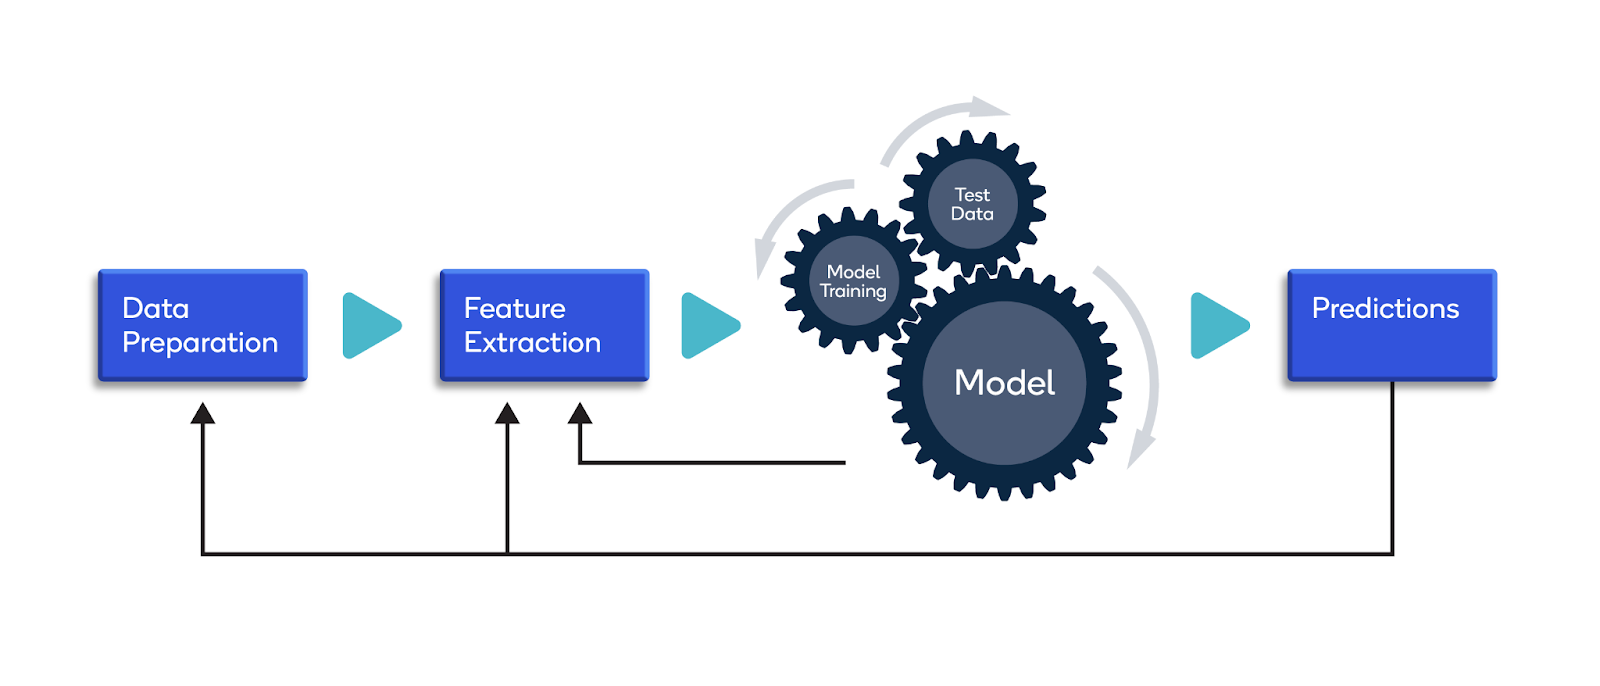
\includegraphics[width=12cm]{./chapter-02-general-ai-information/machine-learning-cv.png}
        \end{center}
        \caption{Machine Learning in Computer Vision ~\cite{mldlcv}}
        \label{fig:mldlcv}
        \end{figure}
    \subsection{Using Deep Learning} 
        Applying deep learning in computer vision is totally different from applying classical machine learning algorithms, firstly,  deep learning requires quantity (huge amounts of image data) over quality to have a robust model with accurate predictions, secondly neural networks saves us the trouble of feature extraction especially when using Convolution Neural Networks ~\cite{machine-learning-full-scale}(Convolution: a mathematical operation on two functions to produce a third function ~\cite{machine-learning-ibm}) this architecture of neural networks is specialized in processing image data and it is built on three primary layers Convolution layer, pooling layer and fully connected layer  ~\cite{mldlcv}.


        \begin{description}
        \item[Convolution layer] \hfill \\
            This layer does most of the hard work by identifying and extracting the features, this is done by applying a filter of random size to blocks of the input image using the dot product between matrices.
        \item[pooling layer] \hfill \\ 
            After the feature extraction resulting from the Convolution layer we need to simplify (by reducing a bloc of values to a single value) the image for easy learning, there are 2 pooling operations max pooling and average pooling.
        \item[fully connected layer] \hfill \\
            It operates on a flattened input, where each input is connected to all the neurons, it is usually found at the end of the network connecting the hidden layers to the output which help in optimizing the class scores.
        \end{description}
        \begin{figure}[htbp]
        \begin{center}
        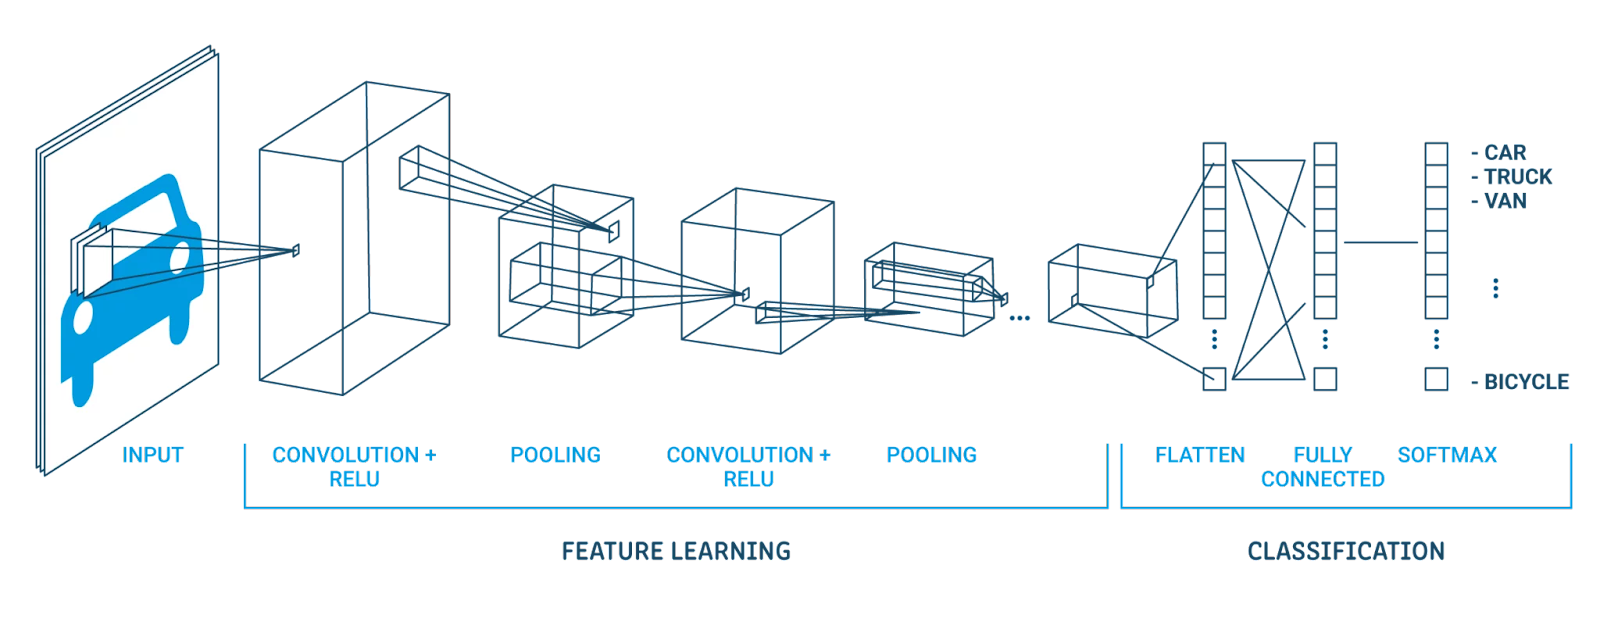
\includegraphics[width=15cm]{./chapter-02-general-ai-information/cnn.png}
        \end{center}
        \caption{Deep Learning in Computer Vision ~\cite{mldlcv}}
        \label{fig:mldlcv}
        \end{figure}
    

    \subsection{Applications of Computer Vision}
        There are a lot of industries using computer vision and these are just a few examples  ~\cite{mldlcv}
        \begin{description}
        \item[medical imaging] \hfill \\ 
            It helps medical professionals interpret faster and diagnose abnormalities.
        \item[law enforcement and security] \hfill \\
            Like in surveillance and authentication.
        \item[self-driving machines] \hfill \\ Like cars and robots.
        \item[gaming] \hfill \\ Augmented reality and virtual reality.
        \item[pattern recognition] \hfill \\
        \end{description}

    \subsection{Some Technologies of Computer Vision}
        Because of the wide utility of computer vision and its benefits there are a lot of libraries and frameworks that facilitates a lot of the hard and repeated tasks, here we mention a few of them  ~\cite{mldlcv}
        \begin{description}
        \item[openCV] \hfill \\ 
            A python library for computer vision,
            \begin{itemize}
                \item super easy to use, 
                \item a huge library of image processing algorithms, 
                \item open source, 
                \item works with GPUs
            \end{itemize}
        \item[Tensorflow] \hfill \\
            made by Google and one of the most popular machine learning frameworks 
            \begin{itemize}
                \item with a wide range of machine/deep learning algorithms, 
                \item open source, 
                \item GPU configured
            \end{itemize}  
        \item[PyTorch] \hfill \\
            made by Facebook, a neural network framework, 
            \begin{itemize}
                \item used a lot by researchers, 
                \item open source, 
                \item works with GPUs
            \end{itemize}
        \item[Caffe] \hfill \\
            a deep learning framework developed by Berkeley AI Research
            \begin{itemize}
                \item open source
                \item c++ based 
                \item easy to use
                \item fast execution 
            \end{itemize}
        \end{description}
